\documentclass[UTF8]{ctexbeamer}

\usetheme{Pittsburgh}
\usefonttheme[onlymath]{serif}

\usepackage{subfig}
\usepackage{multirow}
\usepackage{xcolor,colortbl}
\usepackage{listings}
\usepackage{amsmath}

% Solarized colors
\definecolor{sbase03}{HTML}{002B36}
\definecolor{sbase02}{HTML}{073642}
\definecolor{sbase01}{HTML}{586E75}
\definecolor{sbase00}{HTML}{657B83}
\definecolor{sbase0}{HTML}{839496}
\definecolor{sbase1}{HTML}{93A1A1}
\definecolor{sbase2}{HTML}{EEE8D5}
\definecolor{sbase3}{HTML}{FDF6E3}
\definecolor{syellow}{HTML}{B58900}
\definecolor{sorange}{HTML}{CB4B16}
\definecolor{sred}{HTML}{DC322F}
\definecolor{smagenta}{HTML}{D33682}
\definecolor{sviolet}{HTML}{6C71C4}
\definecolor{sblue}{HTML}{268BD2}
\definecolor{scyan}{HTML}{2AA198}
\definecolor{sgreen}{HTML}{859900}

\lstset{
    % How/what to match
    sensitive=true,
    % Border (above and below)
    frame=lines,
    % Extra margin on line (align with paragraph)
    xleftmargin=\parindent,
    % Put extra space under caption
    belowcaptionskip=1\baselineskip,
    % Colors
    backgroundcolor=\color{sbase3},
    basicstyle=\color{sbase00}\ttfamily,
    keywordstyle=\color{scyan},
    commentstyle=\color{sbase1},
    stringstyle=\color{sblue},
    numberstyle=\color{sviolet},
    identifierstyle=\color{sbase00},
    % Break long lines into multiple lines?
    breaklines=true,
    % Show a character for spaces?
    showstringspaces=false,
    tabsize=2
}


% Title
\title{第6章 离散概率模型}
\author{韩建伟}
\institute{
  信息学院\\
  \texttt{hanjianwei@zjgsu.edu.cn}
}
\date{2019/11/13}

\begin{document}

% Title page
\begin{frame}[plain]
  \titlepage{}
\end{frame}

\begin{frame}{离散概率模型}

  \begin{block}{马尔可夫链}
    系统可以从一个状态转移到另外一个,每个时段转移一次,并且这种向每个可能结果的转移存在一定的概率。
  \end{block}

  \begin{figure}
    \centering
    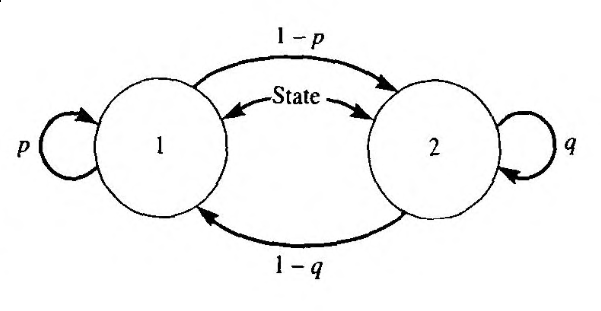
\includegraphics[width=0.6\textwidth{}]{markov.png}
  \end{figure}

\end{frame}

\begin{frame}{再论汽车租赁公司}
  \begin{figure}
    \centering
    \subfloat[转移矩阵]{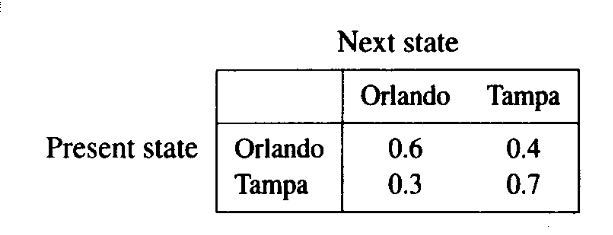
\includegraphics[width=.4\textwidth{}]{transmatrix.png}}
    \subfloat[二状态马尔可夫链]{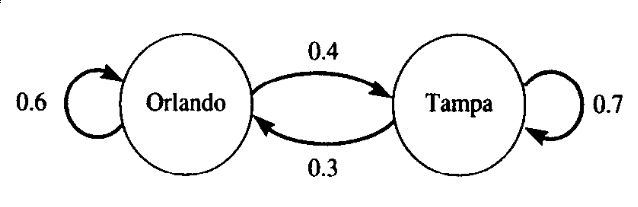
\includegraphics[width=.4\textwidth{}]{transgraph.png}}
  \end{figure}

  \[
  p_{n+1} = 0.6p_n + 0.3q_n
  \]
  \[
  q_{n+1} = 0.4p_n + 0.7q_n
  \]

  \[
  p_k \rightarrow 3/7 = 0.428571
  \]
  \[
  q_k \rightarrow 4/7 = 0.571429
  \]
\end{frame}

\begin{frame}{投票趋势}
  \begin{figure}
    \centering
    \setcounter{subfigure}{0}{}
    \subfloat[转移矩阵]{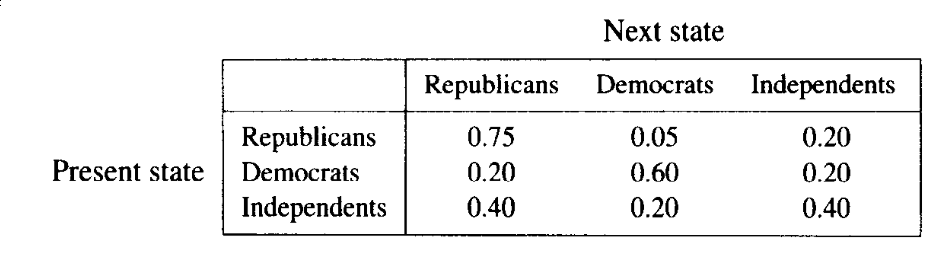
\includegraphics[width=.4\textwidth{}]{votematrix.png}}
    \subfloat[三状态马尔可夫链]{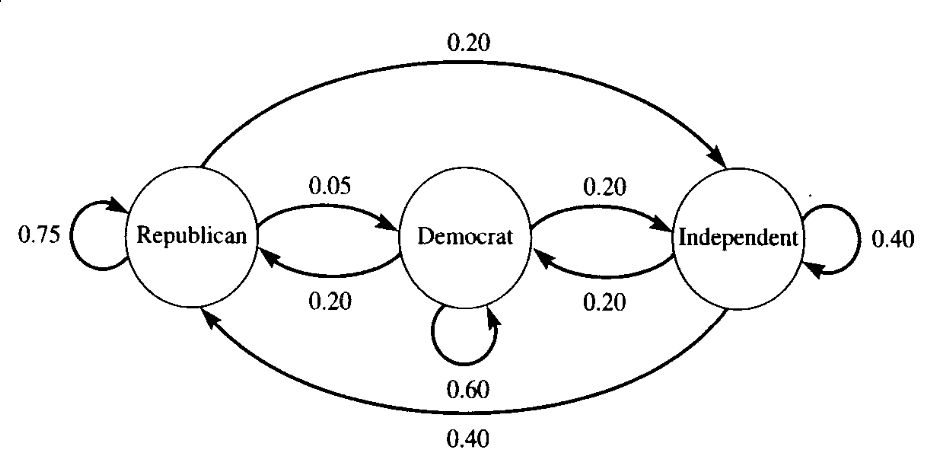
\includegraphics[width=.4\textwidth{}]{votegraph.png}}
  \end{figure}
  \[
  R_{n+1}=0.75R_n+0.20D_n+0.40I_n
  \]
  \[
  D_{n+1}=0.05R_n+0.60D_n+0.20I_n
  \]
  \[
  I_{n+1}=0.20R_n+0.20D_n+0.40I_n
  \]

\end{frame}

\begin{frame}{马尔可夫链}

  \begin{block}{定义}
    \begin{enumerate}
    \item 一个事件有有限多个结果,称为状态,该过程总是这些状态中的一个
    \item 在过程的每个阶段或者时段,一个特定的结果可以从它现在的状态转移到任何其它状态,或者保持原状态
    \item 每个阶段从一个状态转移到其他状态的概率用一个转移矩阵表示,矩阵每行的各个元素在0到1之间,每行的和为1,这些概率只取决于当前状态,而与过去状态无关
    \end{enumerate}
  \end{block}
  
\end{frame}

\begin{frame}{部件和系统的可靠性建模}

  \begin{description}
  \item[$f(t)$] 一个零件、部件或系统在时间$t$内的失效率(概率分布)
  \item[$F(t)$] 相应于$f(t)$的累计分布函数
  \item[$R(t)$] 一个零件、部件或系统的可靠性,$R(t)=1-F(t)$
  \end{description}
  
\end{frame}

\begin{frame}{串联系统}
  \begin{figure}
    \centering
    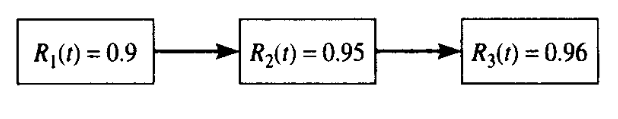
\includegraphics[width=.5\textwidth{}]{nasa.png}
    \caption{NASA宇宙火箭推进系统}
  \end{figure}

  \[
  R_s(t) = R_1(t)R_2(t)R_3(t) = (0.90)(0.95)(0.96) = 0.8208
  \]
  
\end{frame}

\begin{frame}{并联系统}
  \begin{figure}
    \centering
    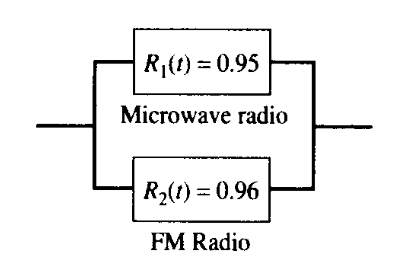
\includegraphics[width=.4\textwidth{}]{nasa-comm.png}
    \caption{NASA宇宙火箭通讯系统}
  \end{figure}

  \[
  R_s(t) = R_1(t) + R_2(t) - R_1(t)R_2(t) = 0.95 + 0.96 - (0.95)(0.96) = 0.998
  \]
  
\end{frame}

\begin{frame}{串并联组合系统}
  \begin{figure}
    \centering
    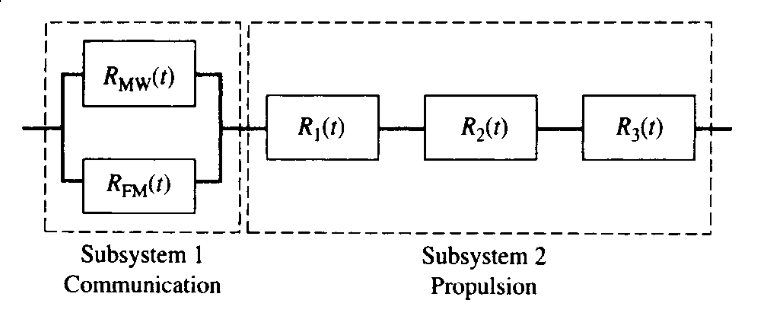
\includegraphics[width=.5\textwidth{}]{nasa-total.png}
    \caption{NASA可控宇宙火箭推进点火系统}
  \end{figure}

  \[
  R_s(t) = R_{s_1}(t)R_{s_2}(t) = (0.998)(0.8208) = 0.8192
  \]
  
\end{frame}

\begin{frame}{线性回归}
  \begin{description}
  \item[线性回归] 一种偏差平方和最小化的统计方法
  \end{description}
  
  \begin{enumerate}
  \item 阐述基本的线性回归模型和它的假设
  \item 定义并解释统计量$R^2$
  \item 利用检查和解释残差散点图对拟合线性回归模型做图形说明
  \end{enumerate}
  
\end{frame}

\begin{frame}{统计量}
  基本的线性回归模型定义为$y_i = ax_i + b$, $y_i$的平均值记作$\bar{y}$,则:

  \begin{description}
  \item[误差平方和] 
    \[
    SSE = \sum_{i=1}^m [y_i - (ax_i + b)]^2
    \]
  \item[总修正平方和] 
    \[
    SST = \sum_{i=1}^m [y_i - \bar{y}]^2
    \]
  \item[回归平方和] 
    \[
    SSR = \sum_{i=1}^m [\bar{y} - (ax_i + b)]^2 = SST - SSE \ge 0
    \]
  \end{description}
  
\end{frame}

\begin{frame}{决定系数}
  \[
  R^2 = 1 - \frac{SSE}{SST}
  \]
  $0 \le R^2 \le 1$, 如果$R^2 = 1$,那么数据精确地与回归直线吻合

  \begin{enumerate}
  \item $R^2$的大小与两个自变量哪一个记作$x$、哪一个记作$y$无关
  \item $R^2$的大小与$x$, $y$的单位无关
  \end{enumerate}

\end{frame}

\begin{frame}{残差}
  残差是实际值和测量值之间的误差:
  \[
  r_i = y_i - f(x_i) = y_i - (ax_i + b)
  \]
  如果将残差对于自变量做图,会得到一些有价值的信息:
  \begin{enumerate}
  \item 残差应随机地分布在与数据精度同量级的、相当小的界限内
  \item 遇到特别大的残差时,应对相应的数据点做进一步的研究,去发现其原因
  \item 残差的模式或者趋势指出了可预测的影响因素仍有待建模,模式的性质常可提供使模型更精确的线索
  \end{enumerate}

  \begin{figure}
    \centering
    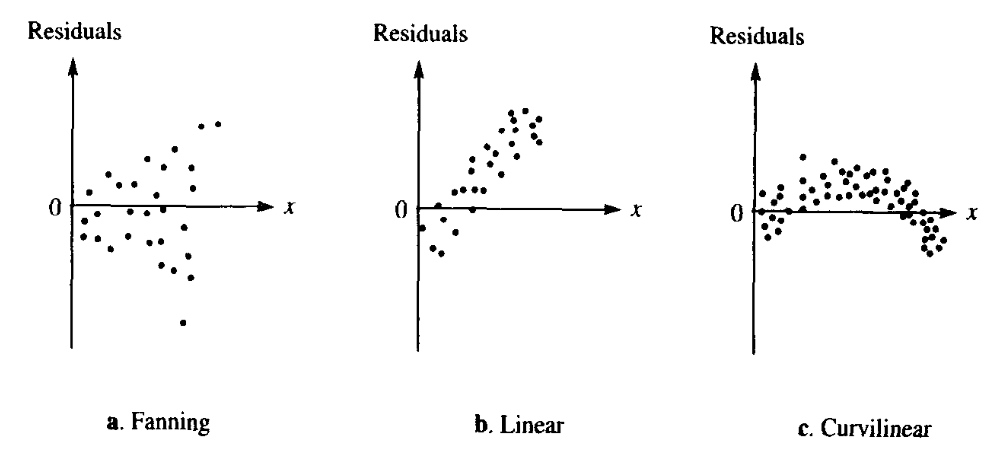
\includegraphics[width=.4\textwidth{}]{error.png}
  \end{figure}

\end{frame}

\begin{frame}{美国黄松}
  \begin{figure}
    \centering
    \setcounter{subfigure}{0}{}
    \subfloat[数据]{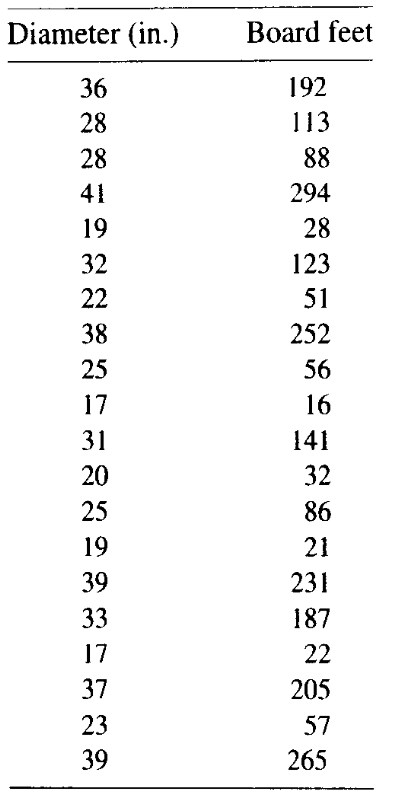
\includegraphics[height=.6\textheight{}]{pine-tab.png}}
    \subfloat[散点图]{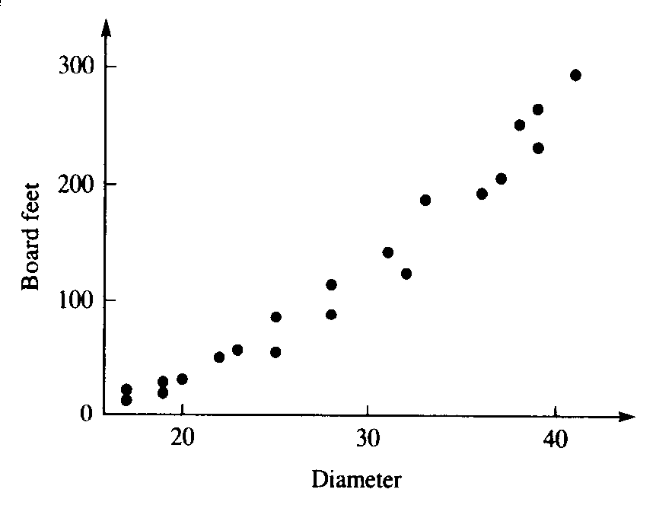
\includegraphics[height=.4\textheight{}]{pine-diameter.png}}
  \end{figure}
\end{frame}

\begin{frame}{建模}
    由几何相似性得到比例关系: 
    \[
    V \propto d^3
    \]
    其中$d$是树的直径,如果假定高度相同,则:
    \[
    V \propto d^2
    \]
    假设树的根部的体积是常数那么上面两个模型进一步精细为:
    \[
    V = ad^3+b
    \]
    \[
    V = \alpha d^2 + \beta
    \]
\end{frame}

\begin{frame}{模型求解及分析}
  用计算机做4个模型的线性回归得到以下解:
    \[
    V = 0.00431d^3
    \]
    \[
    V = 0.00426d^3 + 2.08
    \]
    \[
    V = 0.152d^2
    \]
    \[
    V = 0.194d^2 - 45.7
    \]

    \begin{figure}
      \centering
      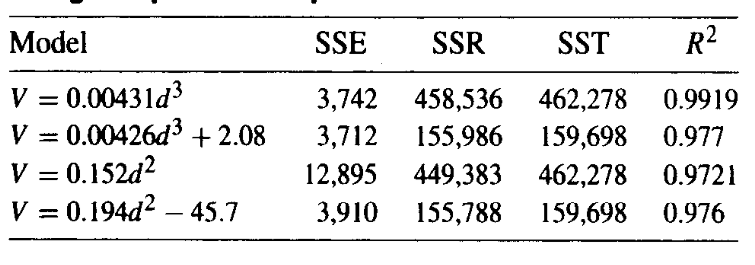
\includegraphics[width=.6\textwidth{}]{pine-regress.png}
      \caption{四个回归模型的主要信息}
    \end{figure}
  
\end{frame}

\begin{frame}{误差分析}

  \begin{figure}
    \centering
    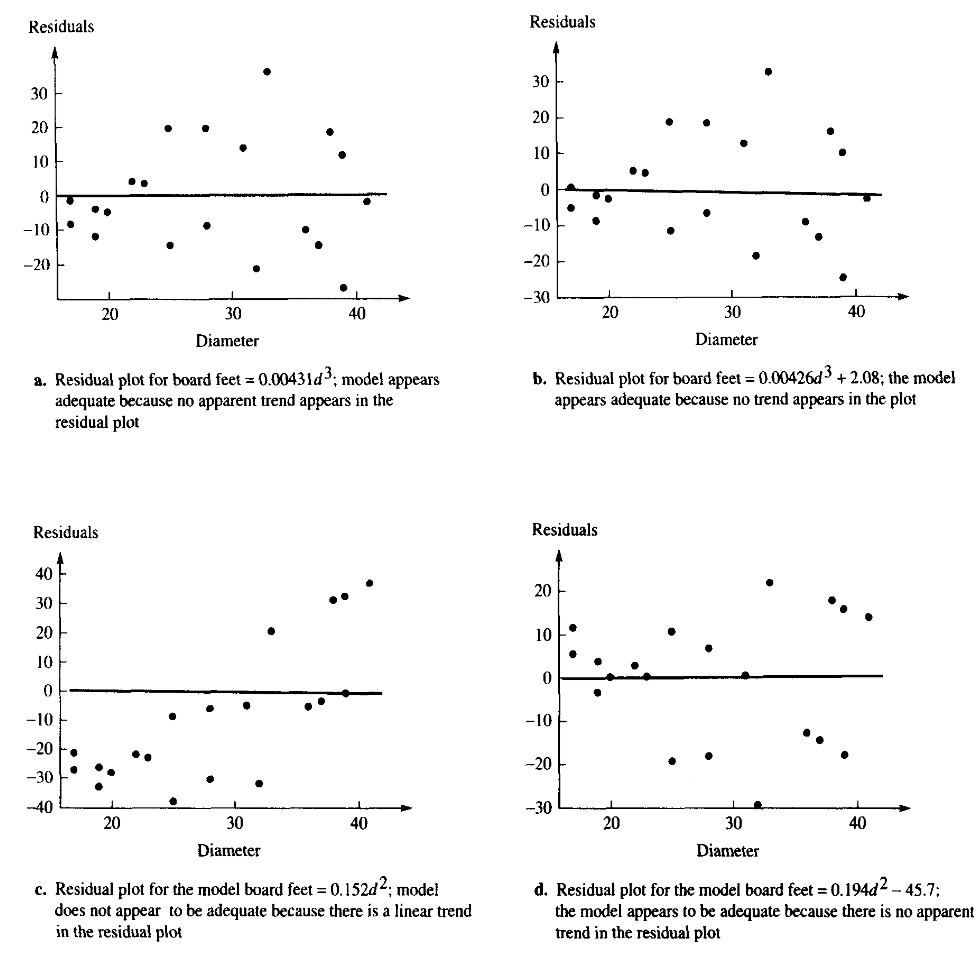
\includegraphics[height=.7\textheight{}]{pine-error.png}
  \end{figure}
  
\end{frame}

\begin{frame}{Matlab中的线性回归}
  \begin{itemize}
  \item \text{[b, bint, r, rint, stats] = regress(y, x)}是线性回归函数
  \item \text{recplot(r, rint)}做残差分析图
  \end{itemize}
\end{frame}

\end{document}

%%% Local Variables: 
%%% TeX-master: t
%%% TeX-engine: xetex
%%% End: 
